\chapter{Измерение качества тематических иерархий}
В обзоре литературы были рассмотрены метрики качества для отдельных тем в тематических моделях. Принятые метрики согласованы с человеческими оценками того, является тема хорошей или плохой.

Тематические иерархии состоят из тем и связей между темами соседних уровней иерархии. Тогда для оценки качества иерархии необходимо измерять не только качество отдельных тем, но и качество отношений "родитель-ребенок"\ в иерархии. В этой работе мы предлагаем несколько метрик качества для ребер иерархии, которые аппроксимируют мнение асессоров о наличии или отсутствии связи между темами.  

\section{Метрики качества ребер иерархии}
\subsection{Метрики на основе лингвистической близости}
 Используем такой же вид метрики качества, что используется при оценке качества отдельных тем, для учета синтагматической или парадигматической родственности топ-токенов темы-родителя и темы-ребенка \cite{Schutze1993}:

$$\mathrm{S}(a, t) = \dfrac{1}{n^2}\sum\limits_{i=1}^{n}\sum\limits_{j=1}^n f(w_i^{(a)}, w_j^{(t)}),$$

Здесь $w_i^{(s)}$ -- это $i$-ый топ-токен некоторой темы $s$. Тема $a \in A$ -- тема $l$-го (родительского) уровня $t\in T$ -- тема $(l+1)$-го (дочернего) уровня, $f(\cdot, \cdot)$ -- мера близости токенов.

Используя ту же меру близости, основанную на совстречаемости токенов, что используется в классической когерентности из \cite{Mimno2011}, получим оценку сходства между темами 

$$\mathrm{S}_{coh}(a, t) = \dfrac{1}{n^2}\sum\limits_{i=1}^n \sum\limits_{j=1}^n \ln \dfrac{D(w^{(a)}_i, w^{(t)}_j) + \varepsilon}{D(w^{(t)}_j)}[w_i^{(a)} \neq w_j^{(t)}].$$ 

Здесь $D(w_1, w_2)$ -- количество документов в некотором корпусе, где слова $w_1$ и $w_2$ встретились вместе, а $D(w)$ -- количество документов, в которых встречается токен $w$.

Используя меру близости из \cite{Nikolenko2016}, основанную на векторных представлениях слов с косинусным расстоянием между векторами, получим метрику 

$$\mathrm{S}_{emb}(a, t) = \dfrac{1}{n^2}\sum\limits_{i=1}^n \sum\limits_{j=1}^n \langle v(w^{(a)}_i), v(w^{(t)}_j)\rangle[w_i^{(a)} \neq w_j^{(t)}],$$ 

где $v(w^{(t)})$ -- вектор, соотвествующий топ-токену $w^{(t)}$ темы $t$ в пространстве word embedding.

\subsection{Метрики на основе вероятностной близости}
В тематической иерархии каждая тема представлена вероятностями токенов в ней, значит можно сравнивать родительские и дочерние темы как вероятностные распределения. Используя две стандартные меры расстояния между распределениями -- расстояние Хеллингера и дивиргенцию Кульбака-Лейблера -- получим следующие метрики:

$$ \mathrm{S}_{Hell}(a, t) = \dfrac{1}{\sqrt{2}} \| \sqrt{p(w|a)} - \sqrt{p(w|t)}\|_2,$$

$$\mathrm{S}_{KL}(a, t) = -D_{KL}(p(w|a)\|p(w|t)).$$

\section{Асессорская разметка ребер иерархии}
Следуя логике, используемой для проверки предлагаемых метрик качества в \cite{Mimno2011, Nikolenko2016}, мы провели асессорский эксперимент, чтобы собрать человеческие оценки качества ребер иерархии.

\subsection{Описанные данных и моделей}
Чтобы собрать пары "родитель-ребенок"\ для аннотации людьми, мы обучили три двухуровневые иерархические тематические модели на трех коллекциях:
\begin{itemize}
\item \textbf{Постнаука (Postnauka.ru)}, научно-популярный интернет-журнал с редактируемыми статьями по широкому спектру тем,
\item \textbf{Хабрахабр (Habrahabr.ru и Geektimes.ru)}, социальные блоги, специализирующиеся на информатике, технологиях и предпринимательстве в сфере IT,
\item \textbf{Элементы (Elementy.ru)}, научно-популярный веб-сайт с особым упором на естественные науки.
\end{itemize}

Коллекции состоят из текстовых документов. Коллекции Постнаука и Хабрахабр вручную протэгированы их авторами или редакторами (каждая статья может содержать несколько тегов).

\begin{table}[h!]
\centering
\begin{tabular}{l|r|r|r|r|r}
& $|D|$ & $|W_1|$ & $|W_2|$ & $|T_1|$ & $|T_2|$ \\
\hline
ПостНаука & 2976  & 43196  & 1799 & 20 & 58 \\
\hline
Хабрахабр & 81076 & 588400 & 77102 & 6 & 15 \\
\hline
Элементы & 2017  & 40452  & -- & 9 & 25 \\
\end{tabular}
\caption{\label{table:tm_datasets}Параметры коллекций. $|D|$ -- размер коллекции, $|W_1|$ -- количество уникальных слов словаря, $|W_2|$ -- количество уникальных тэгов, $|T_1|$ -- количество тем на первом (родительском) уровне, $|T_2|$ -- количество тем на втором (дочернем) уровне.}
\end{table}

\subsection{Постановка задания для асессоров}

Эксперимент проводился на краудсорсинг
платформе Yandex.Toloka. Участвующим асессорам был задан следующий вопрос про каждую пару тем: "Даны темы $T_1$ и $T_2$. Является ли одна из тем подтемой другой?". Были следующие варианты ответа: "$T_1$ - это подтема $T_2$", "$T_2$ - это подтема $T_1$" и "Темы не связаны". Каждая тема $t$ была обозначена 10 топ-токенами из ее распределения вероятностей $p(w|t)$.

После завершения эксперимента первые два варианта ответа были сгруппированы в один ответ «есть связь между темами», поскольку для асессоров часто было трудно отличить тему-родителя от темы-ребенка по наиболее вероятным словам тем. 

\subsection{Контроль качества}
Асессоры были отобраны из состава топ-50\% экспертов Yandex.Toloka по рейтингу, полученному в ходе всех предыдущих заданий, выполненных
экспертом. Перед началом разметки каждый асессор проходил обучение, состоящее из 22 пар тем, которые мы разметили вручную до эксперимента.

Эксперты могли пропустить некоторые задания, если были не уверены в ответе. Асессоры, которые пропустили больше 10 задач подряд отстранялись от участия в эксперименте. Каждому асессору было разрешено разметить не более 125 ребер. 

Каждая пара тем оценивалась пятью разными экспертами.

\subsection{Результаты}
В эксперименте приняли участие 68 асессоров, каждый из которых в среднем оценил около 100 пар тем. Оценка одной пары тем в среднем занимала около 5 секунд.
  В итоге было собрано 6750 оценок 1350 уникальных пар тем.
  
Участники эксперимента были в основном гражданами России и Украины возрастом от 21 до 64 лет.


Для каждой пары тем мы подсчитали, сколько асессоров дали один и тот же ответ (что темы данной пары связаны или не связаны). В нашем случае, для 5 различных асессоров на каждую пару тем, всегда есть решение большинства о том, связаны ли темы. При этом для каждой темы с ответом большинства могут быть согласны 3, 4 или все 5 асессоров. 

\begin{table}[h!]
\centering
\begin{tabular}{r|r|r}
 Уровень согласия & Количество ребер & Процент ребер \\
\hline
3 & 374 & 27.7\% \\
\hline
4 & 468 & 34.7\% \\
\hline
5 & 508 & 37.6\% 
\end{tabular}
\caption{\label{table:agreement}. Согласие асессоров. Уровень согласия -- количество асессоров, согласных с решением большинства. Приведены количество и процент от общего числа ребер, соответствующие каждому уровню согласия.}
\end{table}


\section{Сравнение метрик с асессорскими оценками}

$$y(T_1, T_2) = \text{sign}(\mathrm{S}(T_1, T_2) - w)$$

\begin{table}[h!]
\centering

\begin{tabular}{l|r}
Метрика       & ROC AUC \\
\hline
$\mathrm{S}_{emb}$ &  0.862  \\
\hline
$\mathrm{S}_{Hell}$ &  0.766  \\
\hline
$\mathrm{S}_{KL}$ &  0.755  \\
\hline
$\mathrm{S}_{coh}$ &  0.637  \\
\end{tabular}
\caption{\label{table:metrics_results}Значения ROC AUC для исследуемых метрик.}
\end{table}

\begin{figure}[h!]
	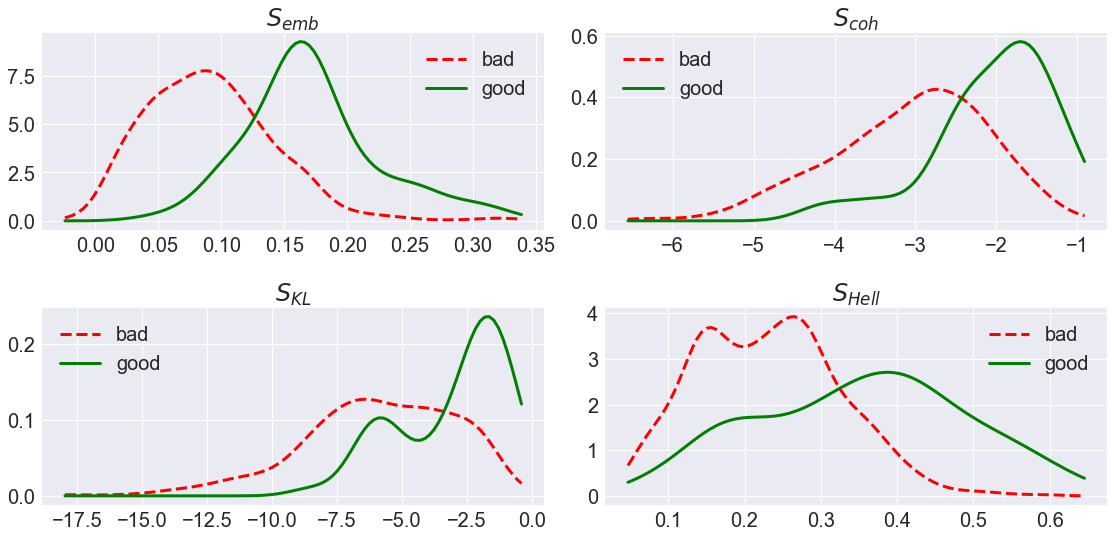
\includegraphics[width=\textwidth]{img/metrics_distr.png}
\end{figure}

\begin{figure}[h!]
	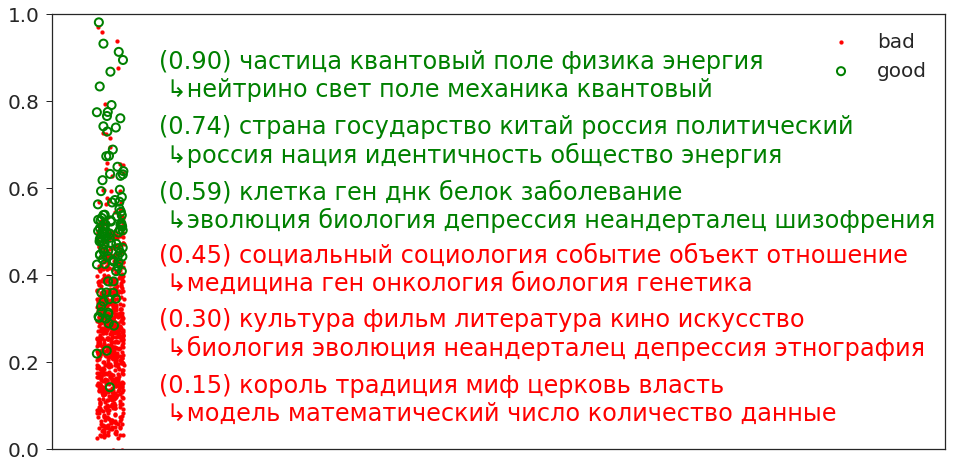
\includegraphics[width=\textwidth]{img/metrics_interpr.png}
\end{figure}

\section{Метрики качества тематических иерархий}




